\section{Introdução}\label{sec:introducao}

% - Qual é a da coisa? (sintese c webaudio)
% - como a coisa funciona? 
%   - como um ou outro fez funcionar
%   - nosso jeito de funcionar

% -----------------------------------------------
 % http://www.charlie-roberts.com/pubs/Gibber_charles_roberts_icmc_2012.pdf


O processamento de sinais digitais de áudio em navegadores de rede, é sumarizado por \cite{w3c_web_2012,roberts_web_2013-,wyse_viability_2014}. \cite{srikumar_tamming_2013} exemplifica a utilização de \emph{nós de áudio}, que podem ser concatenados em um grafo de DSP, como três instâncias de nós diferentes -- \emph{OscilatorNode}, \emph{GainNode}, \emph{DestinationNode} --, na Figura \ref{fig:shime}. Existe um outro nó, \emph{ScriptProcessorNode} que possibilita a customização de funções sonoras. Por exemplo, o \emph{ScriptProcessorNode} pode ser usado para externalizar a(o) improvisador(a) suas próprias customizações de ``nós virtuais'' (funções matemáticas), semelhantes aos \emph{OscilatorNode} e \emph{GainNode} . Esta abordagem foi utilizada no desenvolvimento do \emph{Termpot}.

\begin{figure}[h]
\centering
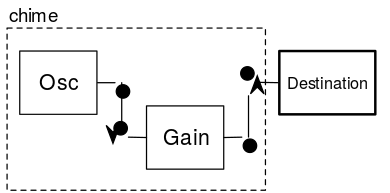
\includegraphics[scale=0.35]{chime.png}
\caption{Estrutura básica de síntese da API webaudio, utilizando instâncias das classes \emph{OscilatorNode}, \emph{GainNode}, \emph{DestinationNode}. \textbf{Fonte}: \cite{srikumar_tamming_2013}.}
\label{fig:shime}
\end{figure}

\section{Trabalho relacionado: GROOVE}

Além da tecnologia \emph{Web Audio}, este artigo envolve uma interpretação do GROOVE -- \emph{Generated Real-time Operations On Voltage-controlled Equipment},  de \cite{mathews_groove_1970}. A compositora Laurie Spiegel (figura \ref{fig:groove}) sumariza a utilização do GROOVE durante a produção de \emph{The Expanding Universe} (1975) \footnote{Disponível em \url{https://www.youtube.com/watch?v=dYUZmsfm4Ww}.}:
\ \\
\begin{quote}
\small{Todas as músicas no GROOVE eram representadas na memória digital como funções abstratas do tempo, séries paralelas de dois pontos, cada ponto sendo um instante no tempo e um valor instantâneo. A taxa de amostragem para essas funções, na maior parte das vezes usada como controle de tensão, era cronometrada por um grande e antiquado oscilador analógico, que era normalmente fixado em 100 Hertz, cada ciclo do oscilador pulsando à frente do código, o computador lia todos dos dispositivos de entrada em tempo real, e reproduzia todas as amostras naquele ponto do tempo em cada uma das funções de tempo. \cite[online]{spiegel_expanding_1975} }\footnote{Tradução de \emph{All music in GROOVE was represented in digital memory as abstract functions of time, parallel series of point pairs, each point being an instant in time and an instantaneous value. The sampling rate for these functions, which would be used mostly as control voltages, was clocked by a big old-fashioned analog oscillator that was usually set to 100 Hertz, each cycle of the oscillator pulsing one run through the code, the computer reading all of the real time input devices and playing of all of the samples at that time point in each of the time functions.}}
\end{quote}

\begin{figure}[!h]
  \begin{center}
  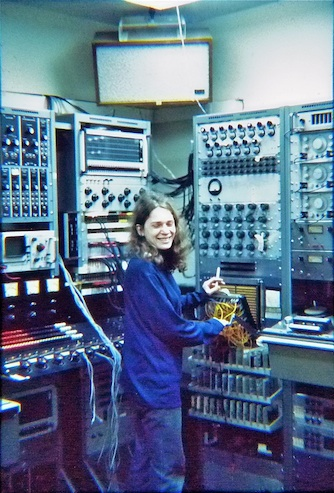
\includegraphics[scale=0.5]{./spiegel.jpg}
  \caption{Laurie Spiegel configurando a saída analógica do GROOVE, durante a produção de \emph{The Expanding Universe}. \textbf{Fonte}: \cite{spiegel_expanding_1975}.}
  \label{fig:groove}
  \end{center}
\end{figure}

\section{Objetivo}

Descrever um programa \emph{web} desenvolvido com base no \emph{ScriptProcessorNode}, e estruturado segundo uma interpretação GROOVE.

%A Seção \ref{sec:trabalhos} deste artigo apresenta os frameworks supracitados e uma breve comparação entre eles.
%A Seção \ref{sec:termpot} apresenta a ferramenta proposta.
%A Seção \ref{sec:resultados} traz os resultados desta pesquisa e a Seção \ref{sec:conclusao} apresenta as conclusões do trabalho até o presente momento.

\section{Metodologia de desenvolvimento}

\begin{inparaenum}[\itshape 1)\upshape]
\item Customização um emulador terminal \emph{Ptty.js} (\url{http://code.patxipierce.com/jquery-plugin/ptty/}).
\item Definição de um ambiente interno, baseado no ambiente \emph{Wavepot} (\url{http://www.wavepot.com}).
\item Definição de comandos deste ambiente interno: inspeção de funções, definição de novas funções, tocar, parar, pausar, gravar e download, criação de controles gráficos (\emph{jQueryUI}) e gravação\footnote{Disponível em \url{https://github.com/mattdiamond/Recorderjs/blob/master/recorderWorker.js}.}.
\end{inparaenum}

